\chapter{Équations dynamiques des systèmes statistiques}

Dans ce chapitre nous analysons la dynamique des systèmes statistiques. L'analyse nous permettra de comprendre comment les transitions de phase, notament certains systèmes subissant une séparation de phase à la transition, se comportent de manière dynamique. L'exemple le plus connu est le modèle d'Ising en absence de champ magnétique, le paramètre d'ordre de la transition étant la magnétisation totale du système. Dans la phase haute température, le système est homogène et sa magnétisation est nulle. En dessous de la température critique, dans le cas où le paramètre d'ordre est conservé (par exemple une dynamique de Kawasaki ou modèle B), le système va localement se séparer en deux phases de magnétisation moyenne opposée séparées par une interface minimisant l'énergie de surface entre les deux phases. 

Dans le cas où le paramètre d'ordre n'est pas conservé (par exemple une dynamique de Glauber ou modèle A), une brisure spontannée de symmétrie fera que l'une des deux phases englobe l'autre, au point de recouvrir tout le système (voir Fig \ref{clusterization}). Dans une transition de phase continue où le point critique est atteint depuis l'état désordonné vers l'état ordonné, les domaines de phase égales sont de taille égale à la longueur de corrélation du système. Dans les transitions de phase telles que celles du modèle d'Ising, cette longueur de corrélation diverge lorsque l'on s'approche de la température critique $T_C$. Dans un système thermodnamique, elle devient infinie, impliquant que le système prend un temps infini pour atteindre l'équilibre thermodynamique : c'est le ralentissement critique. Ce processus de croissance des domaines depuis la phase désordonnée s'appelle le \textit{coarsening} et la théorie de la cinétique d'ordre des phases est la théorie développée pour le comprendre.
Cette thèse s'appuie sur cette théorie afin de déterminer les propriétés statistiques (telles que la position moyenne et la tension superficielle) des interfaces entre deux phases coexistantes.

Les configurations d'équilibre possibles proviennent du compromis entre la minimisation de l'énergie totale et la maximisation de l'entropie. La dynamique hors-équilibre du coarsening qui en résulte peut être étudiée en construisant un modèle qui  minimise l'énergie en fonction du temps, malgré le bruit thermique. Dans la figure \ref{clusterization}, nous montrons un exemple de coarsening dans le cas du modèle d'Ising en fonction du temps. Nous verrons tout au long de ce travail comment les propriétés statistiques sont influencées par l'ensemble thermodynamique dans lequel on se place. Nous nous référons principalement dans ce chapitre aux références \cite{hohenberg_theory_1977,bray_theory_1994,krapivsky_kinetic_2010,halpin-healy_kinetic_1995}.

\begin{figure}[t]
    \centering
    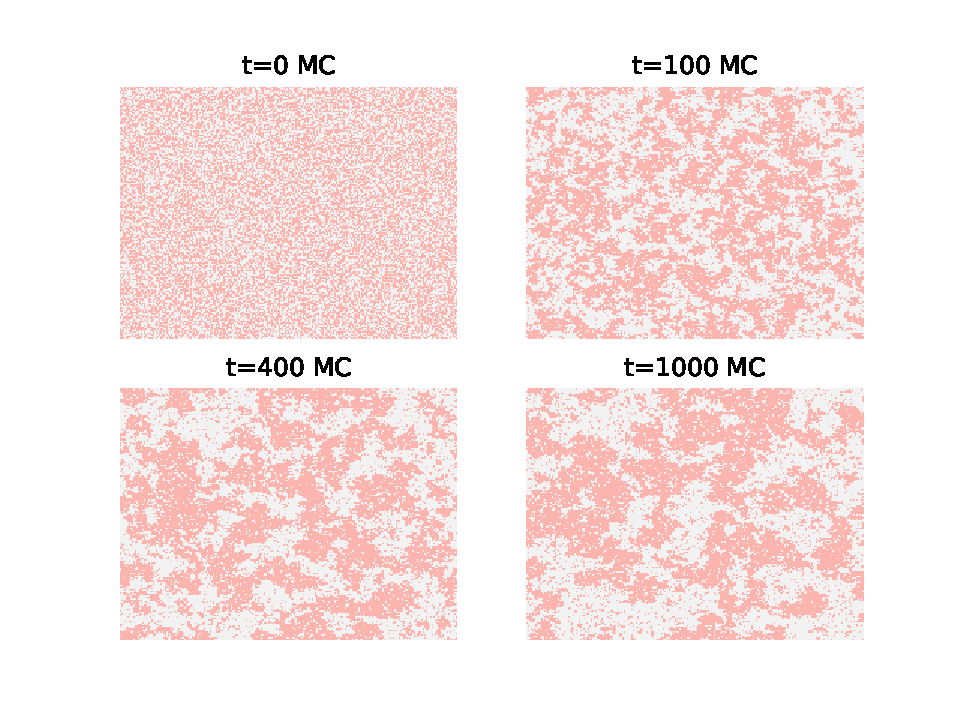
\includegraphics[width=0.9\linewidth]{intro/clusterization.pdf}
    \caption{Phénomène d'aggrégation à partir d'une trempe (\textit{quench}) dans un modèle d'Ising de $T=\infty$ à $T=T_{2D,C}$ \cite{onsager_crystal_1944} pour différents temps en étapes de Monte Carlo, pour un système $600 \times 600$ avec une dynamique non-conservée de Glauber.}
    \label{clusterization}
\end{figure}

La mesure des observables nécessite une connaissance parfaite de la dérivée de la fonction de partition $\mZ$, et donc d'explorer l'espace des phases des configurations du système. Les appareils de mesure possèdent tous une résolution spatiale et temporelle, c'est-à-dire qu'ils mesurent l'état moyen de toutes les particules dans un volume et dans un laps de temps donné. Plus la résolution des appareils de mesure est bonne, et plus la mesure des observables dérivées de la fonction de partition est précise. Si $\Phi(\mx,t)$ est le champ réel de l'observable du système, alors l'appareil, possédant une précision dans le temps et l'espace de $(dt,2dx,2dy,2dz)$ mesure le champ
\begin{align}
    \phi(\mx,t) = \frac{1}{8~ dt~ dx~ dy~ dz} \int_{t-dt}^{t} dt' \int_{x-dx}^{x+dx} dx' \int_{y-dy}^{y+dy} dy' \int_{z-dz}^{z+dz} dz' \Phi(x,y,z,t)
    \label{renormalisation}
\end{align}


%%%%%%%%%%%%%%%%%%%%%%%%%%%%%%%%%
\section{Équation dynamique d'un champ}
%%%%%%%%%%%%%%%%%%%%%%%%%%%%%%%%%

    \subsection{Champ avec un nombre de degrés de liberté fini}
Considérons un système dans l'ensemble canonique d'Hamiltonien  $H(\mq)$ où les $\mq_i$ ($i \in [0,N]$) représentent un nombre fini de degrés de liberté. La fonction de partition est donnée par 
\begin{align}
    Z = \int d\mq \exp(-\beta H(\mq))
\end{align}
avec la probabilité que le système se retrouve dans l'état $\mq$ égale à
\begin{align}
    P_{eq}(\mq) = \frac{\exp(-\beta H(\mq))}{Z}
    \label{eqdis}
\end{align}
À cause du trop grand nombre de degrés de libertés, la fonction de partition est rarement calculable analytiquement. Dans la limite $\beta \to \infty$, l'entropie des états excités devient négligeable, et l'intégrale peut s'approcher par la méthode de Laplace pour l'évaluation des intégrales 
\begin{align}
    Z_{MF}= \exp(-\beta H(\mq^*))
\end{align}
Le champ $\mq^*$ minimise $H$ dont les degrés de liberté sont déterminés par
\begin{align}
    \frac{\partial H}{\partial q_i}|_{\mq={\bf q^*}}=0
\end{align}
À cause du bruit thermique, le système évolue dans le voisinnage de $\mq^*$dans l'espace des configuration : c'est \textbf{le champ moyen}. Dans cette approximation de champ moyen, toute observable est donnée par
\begin{align}
    < f(\mq) > = f(\mq^*)
\end{align}
On considère maintenant l'évolution temporelle du champ réel $\mq$ 
\begin{align}
    \frac{d q_i}{dt} = -L_{ij}\frac{\partial H(\mq)}{ \partial q_j} + \eta_i(t)
    \label{dynamique-langevin}
\end{align}
où $L_{ij}$ est un opérateur matriciel à définir afin que le système respecte la distribution à l'équilibre de Gibbs-Boltzmann,  et $\eta_i(t)$ un bruit blanc gaussien de fonction de corrélation
\begin{align}
   <  \eta_i(t)\eta_j(t') > =   \delta(t-t') \Gamma_{ij}
\end{align}
Le bruit blanc gaussien représente l'effet des fluctuations thermiques sur le système. On considère ici que le temps de corrélation de ces fluctuations est bien plus court que le temps charactéristique de l'évolution temporelle des degrés de liberté $q_i$, ce qui est de plus en plus vrai lorsque l'on se rapproche du point critique\cite{}, à cause du ralentissement critique. Par symmétrie des fonctions de corrélation et de l'équation précédente nous pouvons en déduire que la matrice $\Gamma_{ij}$ doit être symmétrique et ne contenir que des valeurs propres positives.
À $T=0$, le système a tendance à minimiser son énergie, c'est-à-dire que
\begin{align}
    \frac{\partial H(\mq)}{ \partial q_j} = 0
\end{align}
Dans cette limite, l'équation \ref{dynamique-langevin} devient $\frac{d q_i}{dt}=0$, impliquant que le terme $\frac{\partial H(\mq)}{ \partial q_j}$ est le seul responsable de l'évolution du système.
Tant que la matrice $L_{ij}$ est inversible, la dynamique à $T=0$ fera tendre le système vers le minimum global en absence de configurations métastables.
L'équation de Fokker-Planck de la densité de probabilité de la fonction des degrés de liberté $p(\mq,t)$ s'écrit 
\begin{align}
    \frac{\partial p(\mq,t)}{\partial t} = \frac{\partial}{\partial q_i} \left[\frac{1}{2}\Gamma_{ij}                 \frac{\partial p(\mq,t)}{\partial q_i} + p(\mq,t) L_{ij}\frac{\partial H(\mq)}{ \partial q_j}\right]
\end{align}
ou de manière plus concise
\begin{align}
    \frac{\partial p(\mq,t)}{\partial t} +\frac{\partial}{\partial q_i}J_i(\mq,t)=0
    \label{courant}
\end{align}
où  ${\bf J}(\mq,t)$ est le courant de probabilité. Le système respecte l'équilibre de Gibbs-Boltzmann si et seulement si $p(\mq,t)=P_{eq}(\mq)$ (donné par l'équation \ref{eqdis}) et que le courant est nul, c'est-à-dire
\begin{align}
    \left[-\frac{\beta}{2}\Gamma_{ij} + L_{ij}\right]\frac{\partial H(\mq)}{ \partial q_j} = 0
\end{align}
Puisque cette relation est vraie quelque soit l'Hamiltonien considéré, on trouve pour tout système thermodynamique à l'équilibre la relation
\begin{align}
    \Gamma_{ij}= 2 k_B T L_{ij}
\end{align}
avec $k_B$ la constante de Boltzmann.

    \subsection{Théorie statistique des champs}

On considère maintenant un système d'Hamiltonien $H[\phi]$  dépendant d'un champ continu $\phi(\mx)$. Comme précédement, la fonction de partition est donnée par 
\begin{align}
    Z = \int d[\phi] \exp(-\beta H[\phi])
\end{align}
L'intégrale fonctionnelle sur tous les champs $\phi$ peut être prise dans la limite où $\phi$ est définie sur un réseau fini et où l'espacement entre chaque point tend vers $0$.
L'approximation du champ moyen devient maintenant
\begin{align}
    Z _{MF}=  \exp(-\beta H[\phi_{MF}])
\end{align} 
où $\phi_{MF}$ est la solution de champ moyen qui minimise $H$, c'est-à-dire 
\begin{align}
    \frac{\delta H}{\delta\phi(\mx)} = 0
    \label{equi-hamil}
\end{align}

Considérons maintenant l'Hamiltonien 
\begin{align}
    H[\phi] = \int d \mx  \frac{\kappa}{2}[{\boldsymbol \nabla} \phi]^2 + V(\phi)
    \label{hamil-mean-field}
\end{align}
où le premier terme correspond à l'énergie d'interaction cherchant à diminuer les variations au sein du système, et le second terme est un potentiel symmétrique possédant deux minima globaux à basse température à $\pm \phi_C$ responsable de la séparation des phases, et possédant un minimum global à $\phi = 0$ à haute température. 

Par analogie avec le système avec un nombre fini de degré de libertés, on peut écrire l'équation de Langevin 
\begin{align}
    \frac{\partial \phi(\mx)}{\partial t}= -L \frac{\delta H}{\delta \phi(\mx)} + \eta(\mx,t).
\end{align}
avec la fonction de corrélation du bruit blanc gaussien
\begin{align}
    < \eta(\mx,t)\eta(\mx',t)> =\delta(t-t')\Gamma(\mx,\mx')
\end{align}
où  $L$ est un opérateur défini par son action sur la fonction $f$ comme
\begin{align}
    L f(\mx) = \int d\mx' L(\mx,\mx')f(\mx')
\end{align}
et de manière identique pour $\Gamma$.
De la même manière que précédement, on trouve que 
\begin{align} 
    \Gamma(\mx,\mx') =2 k_B T L(\mx,\mx')
\end{align}

Il est possible de choisir l'opérateur $L$ que l'on désire, puisque la distribution de Gibbs-Boltzmann à l'équilibre ne repose que sur la relation entre $L$ et $\Gamma$. 
Halperin et Hohenberg \cite{hohenberg_theory_1977} ont classifié les formes d'opérateurs les plus importants correspondant à des systèmes physiques.

La forme la plus simple est le \textbf{modèle A} donnée par $L(\mx,\mx')=\alpha\delta(\mx-\mx')$ 
\begin{align}
    \frac{\partial \phi(\mx)}{\partial t}= -\alpha \frac{\delta H}{\delta \phi(\mx)} + \eta(\mx,t)
    \label{MA}
\end{align}
de bruit blanc
\begin{align}
    < \eta(\mx,t)\eta(\mx',t)> =2T \alpha \delta(t-t')\delta(\mx-\mx').
\end{align}
On peut voir que la valeur moyenne $\overline \phi(t) = \frac{1}{V}\int d\mx \phi(\mx,t)$ n'est pas conservée. Le modèle A correspond alors à un système dans l'ensemble grand-canonique. Ici, le terme $\alpha$ est un coefficient cinétique décrivant le temps de relaxation du système. 

Un autre modèle est le \textbf{modèle B}, donné par $L(\mx-\mx')= -D{\boldsymbol \nabla}^2 \delta(\mx-{\bf x'})$ où le signe moins est nécessaire pour garantir la positivité de l'opérateur. On obtient l'équation d'évolution
\begin{align}
    \frac{\partial \phi(\mx)}{\partial t}= D{\boldsymbol \nabla}^2 \frac{\delta H}{\delta \phi(\mx)} + \eta(\mx,t)
    \label{MB}
\end{align}
de bruit blanc
\begin{align}
    <\eta(\mx,t)\eta(\mx',t)> =-2TD   \delta(t-t'){\boldsymbol \nabla}^2\delta(\mx-\mx')
\end{align}
En introduisant un bruit blanc vectoriel de composantes $\eta_i(\mx,t)$ tel que 
\begin{align}
    < \eta_i(\mx,t) \eta_i(\mx',t')> =\delta_{ij} \delta(\mx-\mx')\delta(t-t),
\end{align}
où $\delta_{ij}=1$ for $i=j$ et $0$ sinon. On pose 
\begin{align}
    \eta(\mx,t)= {\boldsymbol \nabla}\cdot {\boldsymbol \eta}(\mx,t)
\end{align}
L'équation \ref{MB} devient 
\begin{align}
    \frac{\partial \phi(\mx)}{\partial t}= {\boldsymbol \nabla}\cdot[ D{\boldsymbol \nabla} \frac{\delta H}{\delta \phi(\mx)} + {\boldsymbol\eta}(\mx,t)]
\end{align}
Écrit sous cette forme, il est facile de voir que la valeur moyenne du paramètre d'ordre $\phi$ est conservé dans le temps. Le modèle B correspond à un système dans l'ensemble canonique, utile pour décrire les phénomènes de diffusion et d'accrétion.

À défaut de fluctuations thermiques, les équations \ref{MA} et \ref{MB} s'appellent respectivement les équations Ginzburg-Landau et de Cahn-Hillard \cite{cahn_free_nodate,langer_new_1975,kawasaki_growth_1978} et donnent l'évolution temporelle du champ moyen. 

    \subsection{Modèle $\phi^4$}
    
Le modèle standard des séparations de phase, appelé $\phi^4$ est donné par le potentiel en double-puits de Landau-Ginzburg \cite[§ 45]{l_landau_physique_1990} 
\begin{align}
    V(\phi) = \frac{1}{2} m^2 \phi^2 + \frac{\lambda}{4!} \phi^4
    \label{phi4}
\end{align} 
où $m^2 = T-T_C$. Pour $m^2 \less 0$, ce potentiel symmétrique possède deux minima globaux à $\phi_C = \pm \sqrt{- \frac{6 m^2}{\lambda} } \pm$. Pour $m^2 \ge 0$, ce potentiel possède un minimum global à $\phi_C = 0$. 

Dans les expériences en laboratoire, les systèmes sont souvent couplés à champ magnétique $h(x)$ d'Hamiltonien
\begin{align}
    H_1 &= - \int d^dx h(\mx)\phi(\mx)
    \label{champ-externe}
\end{align}
Comme on le voit dans la figure \ref{double-puits-temperature}, l'ajout d'un champ externe uniforme au potentiel \ref{phi4} favorise l'une des deux phases par rapport à l'autre. La nouvelle fonction de partition est
\begin{align}
    \mZ[h] = \int d [\phi] \exp \left( - \beta \int d^d x \left( \frac{\kappa}{2} ({\boldsymbol \nabla} \phi(\mx))^2 + V(\phi(\mx) \right) + \beta \int d^d x h(\mx) \phi(\mx) \right)
\end{align}

\begin{figure}
    \centering
    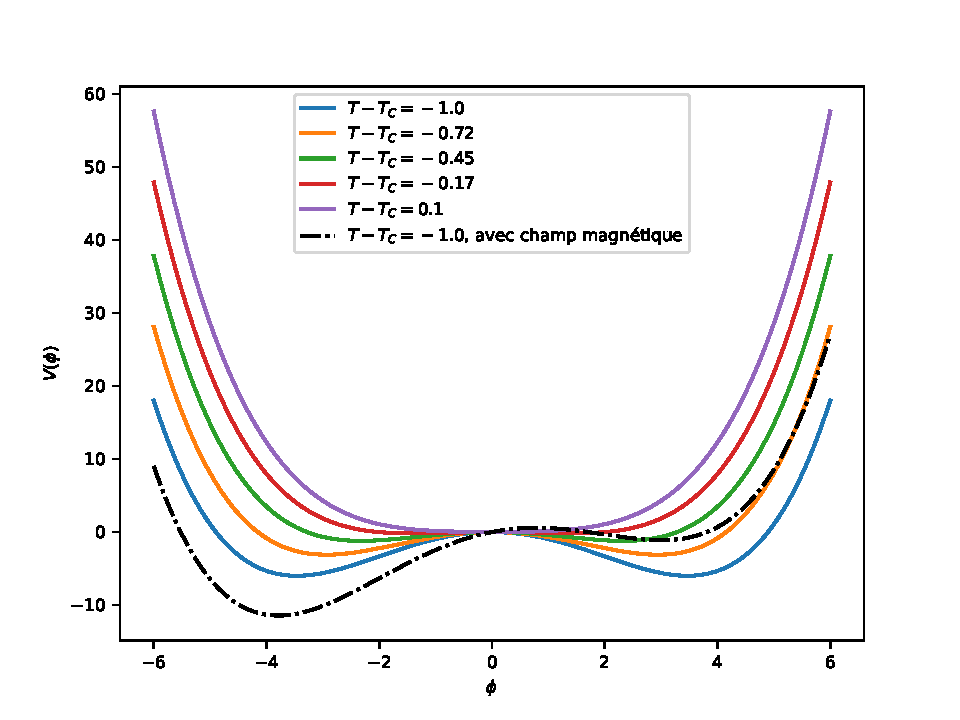
\includegraphics[width=0.6\linewidth]{intro/double-puit-en-fonction-temp.pdf}
    \caption{Potentiel en double-puits \ref{phi4} pour $\lambda=1$ en fonction de la différence entre la température et la température critique avec $m^2 = T-T_C$. Dans la phase ordonnée, les mimina stables sont à $\phi_C =\pm \sqrt{- \frac{6 m^2}{\lambda} } $, pour la phase désordonnée à $\phi_C = 0$. En noir, l'ajout d'un champ magnétique uniforme $h(\mx) = 1$ rend la phase positive métastable.}
    \label{double-puits-temperature}
\end{figure}

La valeur moyenne de $\phi$ est alors
\begin{align}
    <\phi> =  \frac{1}{\mZ[h]} \int d [\phi] \phi(\mx)\exp \left( - \beta \int d^d x \left( \frac{\kappa}{2} ({\boldsymbol \nabla} \phi(\mx))^2 + V(\phi(\mx) \right) + \beta \int d^d x h(\mx) \phi(\mx) \right)
\end{align}
Plaçons-nous maintenant dans la phase désordonnée, où $m^2 \ge 0$ et $\lambda \sim 0$, ce qui nous permet d'avoir une approximation gaussienne. Si on réécrit l'Hamiltonien sous forme d'opérateurs, on obtient 
\begin{align}
    H[\phi] = \frac{1}{2} \int d^d x d^d y \; \phi(\mx) \mL(\mx,\my) \phi(\my) - \int d^d x h(\mx) \phi(\mx)
\end{align}
où l'on a introduit l'opérateur $\mL(\mx,\my) = (m^2 - \kappa {\boldsymbol \nabla}^2) \delta(\mx-\my)$.
La fonction de partition prend maintenant la forme gaussienne
\begin{align}
    \mZ[h] \propto \exp \left(- \frac{\beta}{2} \int d^d x d^d y h(\mx) \mL^{-1}(\mx,\my) h(\my) \right)
\end{align}
où $\mL^{-1}$ est déterminé par 
\begin{align}
    (m^2 - \kappa {\boldsymbol \nabla}_\my^2) \mL^{-1}(\mx,\my) = \delta(\mx-\my)
\end{align}
Par identification avec la fonction de Green $\Gamma(\mx)$ de l'opérateur $m^2 - \kappa {\boldsymbol \nabla}^2$, on obtient que l'énergie libre du modèle gaussien est au final donné par 
\begin{align}
    F[h] = F_0 - \frac{1}{2} \int d^d x d^dy \;  h(\mx) \Gamma(\mx-\my) h(\my)
\end{align}
La transformée de Fourrier de l'équation de la fonction de Green
\begin{align}
    (m^2-\kappa {\boldsymbol \nabla}^2) \Gamma(\mx) = \delta(\mx)
\end{align}
donne
\begin{align}
    \tilde{\Gamma}(\mq) = \frac{1}{\kappa} \frac{1}{\xi^{-2} +  q^2}
\end{align}
Par inversion de la transformée de Fourrier on obtient 
\begin{align}
    \Gamma(\mx) = \frac{1}{\kappa} \int \frac{d^dq}{(2\pi)^d} \frac{\exp(i \mq \cdot \mx)}{\xi^{-2} +  q^2}
    \label{fonction-correl}
\end{align}
où l'on a introduit la longueur de corrélation du système $\xi = \sqrt{\frac{\kappa}{m^2}}$.
Par ailleurs, par différentiation fonctionnelle directe de la fonction de partition, on voit que
\begin{align}
    <\phi(\mx)> = \frac{1}{\mZ[h]} \frac{1}{\beta} \frac{\delta \mZ[H]}{\delta h(\mx)} = \frac{\delta (k_B T \ln \mZ[h])}{\delta h(\mx)} = - \frac{\delta F}{\delta h(\mx)} = \int d^d \my \Gamma(\mx-\my) h(\my)
    \label{moyenne-phi}
\end{align} 
avec l'énergie libre du système  $F[h] = -k_B T \ln(\mZ[h])$. Ce résultat n'est valable que pour $h \neq 0$ ou $h \to 0$. En absence de champ extérieur, la magnétisation est nulle.
De la même manière, on peut démontrer que la fonction de corrélation est égale à 
\begin{align}
    C(\mx,{\bf y}) =  <\phi(\mx)\phi({\bf y})> = \frac{1}{\beta} \frac{\delta <\phi(\mx)>}{\delta h({\bf y})} = \frac{1}{\beta} \Gamma(\mx-\my)
\end{align}
et le facteur de structure
\begin{align}
    S({\bf k},\mq) = < \tilde{\phi}({\bf k})\tilde{\phi}(\mq)> = \frac{(2 \pi)^d}{\beta} \delta({\bf k}-\mq)  \tilde{\Gamma}(\mq)
\end{align}
Dans la phase désordonnée, où $m^2 \less 0$ et $\lambda \neq 0$, l'approximation gaussienne du modèle $\phi^4$ donne le même résultat que \ref{fonction-correl} avec le facteur $m^2$ renormalisé par l'équation auto-consistante \cite[\P 4.3]{bellac_equilibrium_2004}
\begin{align}
    m^2_0 = m^2 + \frac{1}{2} \lambda \int d^d q \frac{1}{m^2_0+\mq^2}
\end{align}

%%%%%%%%%%%%%%%%%%%%%%
    \subsection{Tension superficielle}
%%%%%%%%%%%%%%%%%%%%%%    
En considérant l'Hamiltonien \ref{hamil-mean-field}, l'équation \ref{equi-hamil} devient
\begin{align}
    \frac{\delta H}{\delta \phi(\mx)} = -\kappa {\boldsymbol \nabla}^2 \phi(\mx) + V'(\phi) = 0
    \label{interface}
\end{align}
Puisque le potentiel $V(\phi)$ est supposé symmétrique et possédant deux minima globaux en $\pm \phi_C$,le système tend vers la solution homogène $\phi(\mx) = \pm \phi_C$ correspondant à l'énergie libre $F=H[\phi_C]=0$. Néanmoins, dans le cas où le paramètre d'ordre est conservé
\begin{align}
    \int d \mx \phi(\mx)=0
\end{align}
la solution $\phi(\mx)=\pm \phi_c$ est impossible. Dans ce cas, le système va se séparer localement en plusieurs phases homogènes $\phi(\mx)= \pm \phi_c$. 
Plaçons-nous au voisinage de l'interface entre deux phases, c'est-à-dire que le champ $\phi$ est invariant par translation en $x$ et $y$ mais pas par rapport à $z$, et que la longueur de corrélation $\xi$ est bien plus grande que la taille de l'interface. On considère alors que $\phi(\mx) = \phi_K(z)$ (où $K$ désigne un \textit{kink}) et $\lim_{z\to\\pm\infty}=\pm \phi_c$, ce qui d'après \ref{interface} donne
\begin{align}
    \kappa \phi_K''(z) =  V'(\phi_K)
    \label{kink}
\end{align}
En multipliant de chaque côté par $\phi'_K(z)$ et en utilisant les conditions aux limites, on trouve que 
\begin{align}
    H[\phi_K]=  A\int dz\ \kappa \phi_K'^2(z)
\end{align}
où $A$ est l'aire de la surface du système dans le plan perpendiculaire à la direction $z$. On peut identifier l'intégrale à une énergie libre par unité de surface, c'est à dire la tension superficielle de l'interface $\sigma$ définie par l'équation d'Allen-Cahn \ref{allen_microscopic_1979}
\begin{align}
    \sigma=  \int dz\ \kappa \phi_K'^2(z)
    \label{tension-superficielle}
\end{align}
Il s'ensuit que l'excès d'énergie est localisé au niveau de l'interface, et que la force principale de la croissance des domaines est la courbure du profil de l'interface, puisque l'énergie du système ne peut diminuer que par une réduction de l'aire totale de l'interface. 

Dans le cas du modèle $\phi^4$ définie à l'équation \ref{phi4}, l'équation \ref{kink} devient
\begin{align}
    \kappa \phi_K''(z) = m^2 \phi_K(z) \left( 1 + \phi_C \phi_K(z) ^2 \right)
       \label{eq-interface-glauber}
\end{align}
Dans le modèle, le comportement est seulement déterminé par le ratio entre $m^2$ et $\lambda$. Posons donc sans perte de généralité $\phi_C = 1$. La solution est  
\begin{align}
    \phi_K(z) = \phi_C \tanh \left( \frac{z}{\xi} \right)
       \label{profil-interface-glauber}    
\end{align}
où $\xi = \sqrt{\frac{-2 \kappa}{m^2}}$. Cette longueur de corrélation diverge lorsque $T \to T_C$. On remarque que pluys la longueur de corrélation augmente, plus la dérivée de l'interface est faible, menant à une diminution de la tension superficielle \ref{tension-superficielle}. Aussi, l'étude expérimentale des systèmes quasi-critiques est une porte d'accès pour l'étude des systèmes à ultra basse tension superficielle \cite{hennequin_drop_2006}. De tels systèmes sont extrêmement sensibles aux instabilités hydrodynamiques causées par l'agitation thermique, présentant de nombreuses applications en microfluiidque par exemple \cite{atencia_controlled_2005}. 

%%%%%%%%%%%%%%%%%%%%%%%%%%%%%%%%%
    \section{Effets de taille finie}
    \label{sec-casimir}    
%%%%%%%%%%%%%%%%%%%%%%%%%%%%%%%%%

    \subsection{Hypothese d'invariance d'échelle}

La divergence de la longueur ce corrélation au point critique signifie que les fluctuations existent à toutes les échelles, que ce soit à l'échelle microscopique ou macroscopique. On s'attend alors que toutes les propriétés d'un système critique infini soient similaires. On parle alors d'invariance d'échelle. Dans un système homogène de volume $V$, on décompose l'énergie libre en une partie de bulk $\omega_b$ qui est extensive, et une partie non-analytique $\omega_s$ provenant de la divergence des fluctuations proche du point critique. En posant $t=\frac{T-T_C}{T_C}$ la distance au point critique et $h$ le champ magnétique externe appliqué, on a
\begin{align}
    \Omega(t,h) = V \omega_b(t,h) + V \omega_{na}(t,h)
    \label{decomposition-free-energie}
\end{align}
On s'intéresse maintenant à la partie non-analytique de l'énergie libre. Si l'on procède à une transformation dans le groupe de renormalisation (RG) \cite{amit_field_2005} par une longueur $b$, le groupe de renomalisation nous donne
\begin{align}
    V \omega_{na}(t,h) = V' \omega_{na}(t',h')
\end{align}
avec $b^d V' = V$, $t'=b^{y_1}t$ et $h'=b^{y_2}h$ où $y_1$ et $y_2$ sont des exposants postifs issus de la renormalisation des champs $t$ et $h$. Cela signifie que
\begin{align}
    \omega_{na}(t,h) = \frac{1}{b^d} \omega_{na}(b^{y_1}t, by^{y_2}h)
\end{align}
Posons par simplicité $t \ge 0$, bien que le même argument est généralisable au cas $t \less 0$. La transformation RG de la fonction de corrélation est de la forme
\begin{align}
    C(r,t,h) = \lambda^2(b) C(\frac{r}{b},b^{y_1}t,b^{y_2}h)
\end{align}
On voit que la distance est modifiée par $r' = \frac{r}{b}$. En étudiant le cas particulier $h=0$ et $b^{y_1}t = 1$, on botient que la fonction de corrélation s'écrit comme
\begin{align}
    C(r,t,h) = \lambda^2(t^{-\frac{1}{y_1}}) C(r/t^{-\frac{1}{y_1}},1,0) \simeq f(\frac{r}{\xi})
\end{align}
par définition, ce qui nous donne une longeur de corrélation de la forme 
\begin{align}
    \xi = t^{-\frac{1}{y_1}}
\end{align}
Supposons maintenant que le système est fini dans l'une des directions,  avec des conditions aux bords soit périodiques ou soit fixes. Puisque les modes de fluctuations sont maintenant contraints par la longueur maximale du système $L$, l'hypothèse d'invariance d'échelle n'est plus valable. La nouvelle hypothèse pour un bloc d'aire $A$ et de hauteur $L$ avec $\sqrt{A} := L' \gg L$, l'hypothèse de taille finie (\textit{finite size scaling}) s'écrit 
\begin{align}
   \omega_{na}(t,h,L^{-1}) = \frac{1}{b^d}\omega_{na}(b^{y_1}t,b^{y_2}h,bL^{-1})
   \label{renorma_singu}
\end{align}
Le champ $L^{-1}$ est maintenant un champ relevant dans le langage RG d'exposant $y_L=1$. Le point important à propos  des effest de taille finie, c'est qu'elles lissent la singularité liée à la transition de phase thermodynamique. Dans le cas où $L$ est grand, un développement limité nous donne une extensive et une contribution de surface
\begin{align}
    \omega_{na}(t,h,L^{-1}) = \underbrace{\omega_s(t,h,0)}_{\omega_{ex}}  +\underbrace{L^{-1} \frac{\partial \omega_s(t,h,0)}{\partial x_3}}_{\omega_s}
    \label{decompostion-singu}
\end{align}
où l'on a définit $\omega_{ex}$ comme étant l'énergie libre d'excès dû au confinement des fluctuations, et $\omega_s$ un terme de surface dû aux conditions aux bords. Le second terme donne une contribution à la partie singulière de l'énergie libre de l'ordre de $AL \times L^{-1}$, c'est-à-dire qu'il se comporte comme une tension de surface effective $\gamma$. Par les mêmes arguments RG que précédement, on  trouve que 
\begin{align}
    \gamma \simeq t^{\frac{d-1}{y_1}} = \xi^{-(d-1)}
    \label{temp-xi}
\end{align}
Ce découplage entre un terme de surface et un terme d'excès de bulk n'est strictement valide que dans la limite thermodynamique. Cependant une telle décomposition pour $L$ finie nous permet d'étudier phénomélogiquement le système. Pour $L$ fini, le découplage n'est plus valide, mais on trouve, en posant $b^{y_1}t=1$ dans la version renormalisée de l'équation \ref{renorma_singu}, que
\begin{align}
    \omega_{na}(t,h,L^{-1}) = \frac{1}{L^d} \Theta(\frac{L}{\xi},\xi^{y_2}h)
    \label{theta-universel}
\end{align}
où la fonction $\Theta$ est une fonction analytique appelée fonction d'échelle universelle. Le calcul de cette fonction universelle a premièrement été fait part Hendrik Casimir \cite{h_b_g_casimir_attraction_1948} pour deux plaques conductrices dans le vide, puis par De Gennes et Fisher dans le cas des systèmes critiques \cite{gambassi_casimir_2009}. Sur l'étude de cette fonction universelle, se référer à \cite{gambassi_critical_2009,cardozo_finite_2015}.
Il est possible que plusieurs systèmes physiques différents partagent la même fonction d'échelle universelle mais avec des amplitudes différentes. Ces systèmes possèdent donc le même comportement proche du point. On dit que ces systèmes appartiennent à la même classe d'universalité.
En mettant ensemble les équations \ref{decomposition-free-energie} et \ref{decompostion-singu}, on trouve que l'énergie libre totale du système, en présence de conditions aux bords qui contraignent les fluctuations, est
\begin{align}
    \Omega(t,h,L^{-1}) &= A L \left( \omega_b(t,h) +  \omega_{ex}(t,h,L) \right) + A w_s(t,h) 
    \label{full-decomposition}
\end{align}
Bien sûr, dans la limite où $L\to \infty$, le terme d'excès $\omega_{ex}(t,h,L^{-1}) \to 0$, puisque la contrainte sur les modes de fluctuations est relâchée. 

%%%%%%%%%%%%%%%%%%%%%%%%%%
    \subsection{Pression de séparation et force de Casimir critique}
%%%%%%%%%%%%%%%%%%%%%%%%%%

La décomposition de l'énergie libre en un terme de bulk, un terme de surface et un terme d'excès, a été développée de manière rigoureuse pour les systèmes critiques. Cependant, cette décomposition peut se faire même en absence d'invariance d'échelle, lorsque la taille des fluctuations devient du même ordre de grandeur que la taille du confinement. La dérivée de l'énergie libre totale, divisé par l'aire du système nous donne la pression
\begin{align}
    F(t,h,L) = -\frac{1}{A} \frac{\partial \Omega(t,h,L^{-1})}{\partial L}
\end{align}
Cette pression se retrouve dans les systèmes critiques\cite{degennes} où elle est appelée force de Casimir critique, dans les systèmes classiques - comme les émulsions - où est nommée pression de séparation (\textit{disjoining pressure})  \cite{stubenrauch_disjoining_2003}, et dans les biomembranes \cite{bitbol_fluctuations_2010}.
En utilisant la décomposition \ref{full-decomposition}, on obtient que la force de confinement s'écrit comme
\begin{align}
    F(t,h,L) = - A \omega_b(t,h) - A \frac{\partial(L \omega_{ex}(t,h,L))}{\partial L}
\end{align}
à laquelle on ajoute la relation \ref{theta-universel} pour trouver que la force de Casimir dépend de la fonction d'échelle universelle $\Theta$ selon
\begin{align}
    F(t,h,L) = - A \omega_b(t,h) - A \frac{1}{L^d} \theta(\frac{L}{\xi},\xi^{y_2}h)
\end{align}
où $f_c := -L^{-d} \theta$ est la pression de Casimir,reliée à la fonction d'échelle universelle $\Theta$ par l'équation 
\begin{align}
    \frac{1}{L^d }\theta(\frac{L}{\xi},\xi^{y_2}h) = - \frac{\partial (L^{1-d} \Theta(\frac{L}{\xi},\xi^{y_2}h))}{\partial L}
\end{align}
On rappelle la relation \ref{temp-xi} entre la température réduite et la longueur de corrélation.
Si l'on trouve la force de Casimir, il est alors possible de remonter à la fonction d'échelle universelle \cite{vasilyev_universal_2009}. Cette force de Casimir dépend des conditions aux bords du système \cite{dantchev_casimir_2017,dantchev_exact_2016} ainsi que de l'ensemble thermodynamique dans lequel on se place \cite{gross_critical_2016,rohwer_transient_2017}. 
 Cette force étant une force émergente d'origine entropique, la somme des forces exercées individuellement par chaque particule du système n'est pas égale à la force totale appliquée sur le système\cite{paladugu_nonadditivity_2016}.

La détection expérimentale de ce phénomène se fait traditionnellement dans des fluides binaires par \textit{Total Internal Reflection Microscopy} (TIRM) \cite{fukuto_critical_2005,hertlein_direct_2008,gambassi_critical_2009,edison_critical_2015-1}. La méthode consiste à mesurer le potentiel d'une sphère flottant sur un fluide binaire critique reposant sur une plaque. Cette sphère et cette plaque sont traitées chimiquement afin de favoriser l'une des deux phases à leu voisinage. Ainsi il est possible de créer des conditions aux bords $(++)$, $(+-)$ ou $(--)$ qui modifient la forme de la fonction universelle \ref{theta-universel}. À l'inverse, il est possible de mesurer la force de Casimir \cite{nguyen_controlling_2013} afin d'étudier les transitions de phases colloïdales.



%%%%%%%%%%%%%%%%%%%%%%%%%%
    \subsection{Intégration sur le paramètre d'ordre}
%%%%%%%%%%%%%%%%%%%%%%%%%%    
{\color{red} mettre dans le chapitre 3. C'est une méthode numérique que j'ai utilisé.}
Afin d'isoler la force de Casimir du terme de volume dans la force de confinement, il convient de retirer la force de confinement d'un système de taille différente. Ainsi, pour deux systèmes de taille $L_1 \less L_2$, on a 
\begin{align}
    F(t,h,L_1) - F(t,h,L_2) = f_c(t,h,L_1) - f_c(t,h,L_2) =  - \frac{\partial \Omega(t,h,L_1)}{\partial L}  + \frac{\partial \Omega(t,h,L_2)}{\partial L} 
\end{align}
Puisque le surplus d'énergie dû au confinement est nul lorsque $L_2\to \infty$, on obtient une approximation sur la force de Casimir lorsque $\frac{L_1^d}{L_2^d} \ll 1$ 
\begin{align}
    f_c(t,h,L_1) \simeq  \frac{\partial \Omega(t,h,L_2)}{\partial L}  - \frac{\partial \Omega(t,h,L_1)}{\partial L} 
    \label{casimir-diff-omega}   
\end{align}

Or, nous savons grâce à l'équation \ref{moyenne-phi} que dans le cas d'un champ magnétique uniforme $h(\mx)$, la moyenne du paramètre d'ordre est reliée à l'énergie libre par
\begin{align}
    <\phi(\mx)>(t,h,L) = - \frac{\delta \Omega(t,h,L)}{\delta h(\mx)}
\end{align} 
Si on pose $h(\mx) = h$, alors il est possible d'obtenir une différence entre deux énergies libres à champs magnétiques différents \cite{lopes_cardozo_critical_2014} 
\begin{align}
    \Delta \Omega = \Omega(t,h_1,L) - \Omega(t,h_2,L) = - \int_{h_1}^{h_2} <\phi(\mx)>(t,h,L) dh
    \label{integration-cardozo}
\end{align}
Dans le cas où l'on connait la configuration lorsque $h_2 \to \infty$ ou $h_1 \to 0$, il est possible de mesurer directement l'énergie libre d'un système pour n'importe quelle température et taille en intégrant selon \ref{integration-cardozo}. Dans le cas où $h_2 \to \infty$, le potentiel en double-puit \ref{phi4} ne possède qu'un seul minimum, l'énergie libre d'un tel système est alors uniquement lié à l'énergie libre du volume.
La différence \ref{integration-cardozo} contient donc toute l'information nécessaire afin de mesurer la force de Casimir. On peut alors calculer la dérivée \ref{casimir-diff-omega} avec
\begin{align}
    dL \frac{\partial \Omega(t,h,L)}{\partial L} = \Delta \Omega(t,h,L)-\Delta \Omega(t,h,L-dL)
\end{align}

%%%%%%%%%%%%%%%%%%%%%%
    \section{Modèles d'interface}
%%%%%%%%%%%%%%%%%%%%%%
La phase désordonnée, où cohabitent la phase 1 et la phase 2, est inhomogène, avec des gouttes ou des digitations. Afin d'étudier les fluctuations au niveau des interfaces entre les phases, nous mettons au point un modèle effectif d'interfaces. Le modèle le plus simple est de considérer que l'interface est définie par une hauteur $h(\mr)$, avec $\mx := (\mr,z)$. On suppose également que $h(\mx)=h(\mr)$.  
On va maintenant poser les équations de la dynamique de la hauteur de l'interface à partir des équations de la théorie statistique des champs. On suppose que les phases sont séparées selon l'axe $z$ et que la hauteur moyenne de l'interface se trouve à $z=0$. L'approximation de l'interface nous permet alors de poser le champ $\phi$ comme étant égal à 
\begin{align}
    \phi(\mr,z,t) = f(z-h(\mr,t))
    \label{hans}
\end{align}
où $f(z)=\phi_K(z)$ est la solution kink du champ moyen \ref{kink}, et $f(z \to -\infty) = \phi_1$ et $f(z \to -\infty) = \phi_2$
L'Hamiltonien considérer est l'Hamiltonien de Landau-Ginzburg \ref{hamil-mean-field}
\begin{align}
    H[\phi] = \int d \mx  \frac{\kappa}{2}[{\boldsymbol \nabla} \phi]^2 + V(\phi)
\end{align}
D'un autre côté, l'Hamiltonien d'une interface libre décrit l'énergie de la surface totale $A$ uniquement, c'est-à-dire que l'on peut trouver un Hamiltonien effectif
\begin{align}
    H[h] = \sigma \int_A d \mr\sqrt{1+[\nabla h]^2}
\end{align}
où l'integrale est fait sur tout le plan perpendiculaire à l'axe $z$ d'aire $A$. Lorsque les fluctuations de l'interface sont faibles, le développement limité au second ordre nous donne
\begin{align}
    H[h]= A\sigma +\frac{\sigma}{2} \int_A d \mr \ [\nabla h]^2
\end{align}
Le premier terme est indépendant de la hauteur. On peut donc réécrire l'Hamiltonien sous la forme d'un Hamiltonien effectif
\begin{align}
    H_{eff} [h]= \frac{\sigma}{2} \int_A d \mr\  [\nabla h]^2
    \label{heff}
\end{align}


%%%%%%%%%%%%%%%%%
    \subsection{Modèle A}
%%%%%%%%%%%%%%%%%
Pou rappel, l'équation de la dynamiqu du champ dans le modèle A s'écrit
\begin{align}
    \frac{\partial \phi(\mx)}{\partial t}= -\alpha \frac{\delta H}{\delta \phi(\mx)} + \eta(\mx,t)
    \label{ma2}
\end{align}
En utilisant le fait que 
\begin{align*}
\frac{\partial f(z-h(\mr,t))}{\partial t}&= -f'(z-h(\mr,t))\frac{\partial h(\mr,t)}{\partial t} \nn
\nabla f(z-h(\mr,t))&= [{\bf e}_z-\nabla h(\mr,t)]f'(z-h(\mr,t))  \nn
\nabla^2 f(z-h(\mr,t))&= f''(z-h(\mr,t))- \nabla^2 h(\mr,t)f'(z-h(\mr,t))+ [\nabla h(\mr,t)]^2 
f''(z-h(\mr,t))
\end{align*}
on introduit l'approximation \ref{hans} dans l'équation de champ moyen afin de trouver
\begin{align}
    -f'(z-h(\mr,t)) \frac{\partial h(\mr,t)}{\partial t} =& 
    \alpha\kappa\times \left[f''(z-h(\mr,t))- \nabla^2 h(\mr,t)f'(z-h(\mr,t))+ [\nabla h(\mr,t)]^2 f''(z-h(\mr,t))\right] \nn
    &- \alpha V'(f'(z-h(\mr,t))) + \eta(\mr,z,t).
\end{align}
En multipliant de part et d'autre l'équation par $f'(z-h(\mr,t))$ et une introduisant le changement de variable $\zeta=z-h(\mr,t)$, on intègre $\zeta$ sur $[-\infty,\infty]$. 
Puisuque $f(\zeta \to \pm \infty)=\pm \phi_c$ et que $V(\phi_c)=V(-\phi_c)=0$, on obtient deux identités supplémentaires
\begin{align}
    \int_{-\infty}^\infty d\zeta f'(\zeta)f''(\zeta) &= [\frac{1}{2}f'^2(\zeta)]_{-\infty}^\infty =0\\
    \int_{-\infty}^\infty d\zeta f'(\zeta) V'(f) &= \int_{-\infty}^\infty d\zeta\frac{d V(f)}{d\zeta}= [V(f(\zeta))]_{-\infty}^\infty=0
\end{align} 
Les termes non nuls dans l'équation \ref{ma2} sont donc
\begin{align}
    -\int_{-\infty}^\infty f'^2(\zeta)d\zeta\ \frac{\partial h(\mr,t)}{\partial t}
    = -\alpha\int_{-\infty}^\infty f'^2(\zeta)d\zeta \ \kappa \nabla^2 h(\mr,t) + \int_{-\infty}^\infty d\zeta \eta(\mr,\zeta+ h(\mr,t))f'(\zeta)
\end{align}
En utilisant l'estimation de Cahn-Hilliard pour la tension superficielle \ref{tension-superficielle}, on obtient 
\begin{align}
    \frac{\sigma}{\kappa} \frac{\partial h(\mr,t)}{\partial t} = \alpha\sigma \nabla^2 h(\mr,t) +\xi(\mr,t),
\end{align}
avec le bruit  
\begin{align}
    \xi(\mr,t)= \int_{-\infty}^\infty d\zeta \eta(\mr,\zeta+ h(\mr,t))f'(\zeta)
\end{align}
Ce bruit est de moyenne nulle et sa fonction de corrélation est
\begin{align}
    < \xi(\mr,t)\xi(\mr',t') > &=2\alpha T\delta(t-t')\delta(\mr-\mr')\int_{-\infty}^\infty d\zeta d\zeta' \delta(\zeta-\zeta')f'(\zeta)f'(\zeta')\nn
    &= 2\alpha T\delta(t-t')\delta(\mr-\mr')\int_{-\infty}^\infty d\zeta f'^2(\zeta) \nn
    &= \frac{2\alpha T\sigma}{\kappa}\delta(t-t')\delta(\mr-\mr')
\end{align}
On obtient 
\begin{align}
    \frac{\partial h(\mr,t)}{\partial t}= \kappa\alpha \nabla^2 h(\mr,t) + \eta(\mr,t)
\end{align}
où 
\begin{align}
    < \eta(\mr,t)\eta(\mr',t') > = \frac{2\alpha T\kappa}{\sigma}\delta(t-t')\delta(\mr-\mr')
\end{align}
En posant $\alpha' = \frac{\kappa\alpha}{\sigma}$, on obtient finalement que 
\begin{align}
    \frac{\partial h(\mr,t)}{\partial t}= \alpha' \sigma\nabla^2 h(\mr,t) + \eta(\mr,t).
\end{align}
Cette équation est la même forme que l'équation du modèle A pour la hauteur de l'interface. Le potentiel $V(\phi)$ étant responsable de la séparation de phase uniquement, il est normal de ne pas le retrouver dans l'équation finale, où l'on étudie un modèle d'interface. En utilisant l'Hamiltonien effectif \ref{heff}, on obtient l'équation d'Edwards-Wilkinson \cite{edwards_surface_1982}
\begin{align}
    \frac{\partial h(\mr,t)}{\partial t}= -\alpha' \frac{\delta H_{eff}[h]}{\delta h(\mr)} + \eta(\mr,t),
    \label{ew}
\end{align}
avec
\begin{align}
    < \eta(\mr,t)\eta(\mr',t')>= 2T\alpha'\delta(t-t').
\end{align}
Cette équation est consistante avec l'idée de décrire la surface de l'interface en termes d'une hauteur variable avec une énergie donnée par une tension de surface.
%
%The equation \eqref{ew} is known as the Edwards-Wilkinson equation. We can use this equation to determine how the domains of a coarsening systems grow at low temperatures. To do this we ignore the noise term and assume that at $t=0$ the correlations of the height are short range so
%\begin{align}
%C(\mr-\mr',0)= < h(\mr,0)h(\mr',0)> =C_0 \delta(\mr-\mr').
%\end{align}
%In Fourier space the noiseless Edwards-Wilkinson equation becomes
%\begin{align}
%\frac{\partial\tilde h({\bf k},t)}{\partial t} = -\alpha'\sigma \tilde h({\bf k},t) ,
%\end{align}
%and so we find
%\begin{align}
%\tilde h({\bf k},t) = h({\bf k},0)\exp(-\alpha'\sigma{\bf k}^2 t).
%\end{align}
%We thus find 
%\begin{align}
%< \tilde h({\bf k},t)\tilde h({\bf k}',t')> = < h({\bf k},0)h({\bf k}',0)> \exp(-\alpha'\sigma[k^2+k'^2] t).
%\end{align}
%Now recall that if 
%\begin{align}
%<  h(\mr,t) h(\mr',t')> =C(\mr-\mr',t)
%\end{align}
%then
%\begin{align}
%< \tilde h({\bf k},t)\tilde h({\bf k}',t')>= (2\pi)^d \delta({\bf k}+{\bf k}') \tilde C({\bf k},t),
%\end{align}
%where 
%\begin{align}
%\tilde C({\bf k},t)= \int d\mr \exp(-i{\bf k}\cdot \mr)C(\mr,t),
%\end{align}
%is the Fourier transform of the correlation function which is a function of a single position due to invariance by translation in space, and $d$ is the dimension of space (so here $d=2$ for a surface in 3d space and $d=1$ for a surface in a 2d space). Putting all this together gives
%\begin{align}
%\tilde C({\bf k},t)= C_0 \exp(-2\alpha'\sigma k^2 t).
%\end{align}
%Inverting the Fourier transform gives
%\begin{align}
%C(\mr,t)= \frac{C_0}{(8\pi \alpha'\sigma t)^{\frac{d}{2}}} \exp(-\frac{\mr^2}{16\pi \alpha'\sigma t}).
%\end{align}
%From this we see that if $C(\mr,t)\sim g(\frac{\mr}{\ell(t)})r(t)$ then the length scale $\ell(t)\sim t^{\frac{1}{2}}$, this agrees with what we found in the Ising model under Glauber dynamics, where the growth exponent is also given by $z=\frac{1}{2}$.
%\\
%%%%%%%%%%%%%%%%%
    \subsection{Modèle B}
%%%%%%%%%%%%%%%%%
On propose de refaire le même calcul d'interface avec l'équation du Modèle B \ref{MB} :
\begin{align}
    -\nabla^{-2} \frac{\partial\phi(\mx,t)}{\partial t} = -D \frac{\delta H}{\delta \phi(\mx)}+ \theta(\mx,t)
\end{align}
où $-\nabla^{-2}$ représente la fonction de Green $G$ qui obéit à
\begin{align}
    \nabla^2 G(\mx-{\bf x'}) = -\delta(\mx-\mx')
\end{align}
et
\begin{align}
    \theta(\mx,t)=-\nabla^{-2}\eta(\mx,t)= \int d\mx'G(\mx-{\bf x'})\eta(\mx,t)
\end{align}
La fonction de corrélation de ce bruit est donné par 
\begin{align}
< \theta(\mx,t)\theta({\bf y},t')> &=-2DT\delta(t-t') \int d\mx'G(\mx-{\bf x'})d{\bf y}'G({\bf y}-{\bf y'})\nabla^2\delta(\mx'-{\bf y}') \nn
&= -2DT\delta(t-t') \int d\mx'G(\mx-{\bf x'})d{\bf y}'\nabla^2G({\bf y}-{\bf y'})\delta(\mx'-{\bf y}') \nn
&= 2DT\delta(t-t') G(\mx-{\bf y}).
\end{align}
Comme précédement, on multiplie l'équation de chaque côté par $f'(z-h(\mr,t))$ puis on intégre $z$ sur$[-\infty,\infty]$ pour trouver 
\begin{align}
-\int dz f'(z-h(\mr,t))\int dz'd\mr'\  G(z-z',\mr-\mr') f'(z'-h(\mr',t))\frac{\partial h(\mr',t)}{\partial t} = -D\sigma \nabla^2 h(\mr,t) + \chi(\mr,t)
\end{align}
avec le bruit
\begin{align}
    \chi(\mr,t)= \int dz f'(z-h(\mr,t)) \theta(\mr,z,t)
\end{align}
En suppose maintenant que les fluctuations de l'interface sont concentrées autour de $0$, ce qui nous permet de faire ne garder que les termes à l'ordre $0$, ce qui nous donne
\begin{align}
    -\int dz \ f'(z)\int dz'd\mr'\  G(z-z',\mr-\mr') f'(z')\frac{\partial h(\mr',t)}{\partial t} = -D\sigma \nabla^2 h(\mr,t) + \chi(\mr,t)
\end{align}
avec le bruit donné par 
\begin{align}
    \chi(\mr,t)= \int dz\  f'(z) \theta(\mr,z',t)
\end{align}
Cette équation linéaire peut maintenant subir une transformation de Fourier dans le plan $\mr$, ce qui nous donne
\begin{align}
    -\int dz \ f'(z)\int dz'd\mr'\ \tilde G(z-z',{\bf k}) f'(z')\frac{\partial\tilde h({\bf k},t)}{\partial t} = 
Dk^2\sigma \tilde h({\bf k},t) + \tilde \chi({\bf k},t)
    \label{bstep}
\end{align}
La transformée de Fourier de $G$ dans le plan $\mr$ suit
\begin{align}
    \frac{d^2 \tilde G(z-z',{\bf k} )}{dz^2}-k^2 \tilde G(z-z',{\bf k} )=-\delta(z-z')
\end{align}
dont la solution avec la condition au bord $\tilde G(z-z',{\bf k} )\to 0$ lorsque $|z-z'|\to\infty$)  est
\begin{align}
    \tilde G(z-z',{\bf k}) = \frac{\exp(-k|z-z'|)}{2k}
\end{align}
avec $k=|{\bf k}|$. On suppose maintenant que l'interface est abrupte, c'est-à-dire que $f(z) = 2\phi_c \delta(z)$, qui est la limite $\xi \to 0$ de la solution \ref{kink}. On obtient
\begin{align}
    -4\phi_c^2 \tilde G(0,k) \frac{\partial h({\bf k},t)}{\partial t} = Dk^2\sigma  h(\mr,t) + \tilde \chi({\bf k},t)
\end{align}
que l'on réécrit comme
\begin{align}
    \frac{\partial \tilde h({\bf k},t)}{\partial t} = -\frac{Dk^3\sigma}{2\phi_c^2} \tilde h({\bf k},t) + \tilde \xi({\bf k},t)
\end{align}
avec
\begin{align}
    \tilde \xi({\bf k},t)= - \frac{k}{2\phi_c^2}\tilde \chi({\bf k},t)=  - \frac{k}{2\phi_c^2} \int dz\  f'(z) \tilde\theta({\bf k},z,t)
\end{align}
La fonction de corrélation de $\tilde \theta({\bf k},t)$ est
\begin{align}
    < \theta({\bf k},t)\theta({\bf k}',t')> = 2DT(2\pi)^d \delta(t-t') \delta({\bf k}+{\bf k'}) \tilde G(z-z',k)
\end{align}
ce qui nous donne
\begin{align}
    < \chi({\bf k},t)\chi({\bf k}',t')>  &= 2DT(2\pi)^d \delta(t-t') \delta({\bf k}+{\bf k'}) \int dz dz' f(z) f(z') \tilde G(z-z',k) \nn
 &= 2DT(2\pi)^d \delta(t-t') \delta({\bf k}+{\bf k'}) \frac{2\phi_c^2}{k}
\end{align}
où l'on a utilisé l'approximation de l'interface abrupte pour passer de la première à la seconde ligne, ce qui nous donne
\begin{align}
    < \xi({\bf k},t)\xi({\bf k}',t')> = 2DT(2\pi)^d \delta(t-t') \delta({\bf k}+{\bf k'}) \frac{k}{2\phi_c^2}
\end{align}
L'équation finale de la dynamique de l'interface pour le modèle B dans l'espace de Fourier est
\begin{align}
    \frac{\partial h({\bf k},t)}{\partial t} = -\frac{Dk^3\sigma}{2\phi_c^2} \tilde h({\bf k},t) + \tilde \xi({\bf k},t)
    \label{modBFT}
\end{align}
On obtient au final, dans l'espace réel, 
\begin{align}
    \frac{\partial h(\mx)}{\partial t}= -L \frac{\delta H_{eff}}{\delta h (\mx)} + \xi(\mx,t)
\end{align}
où l'opérateur $L$ est défini dans l'espace de Fourier par
\begin{align}
    \tilde L({\bf k}) = \frac{Dk}{2\phi_c^2}
    \label{op-mb}
\end{align}
%Now if we look at Eq. \eqref{modBFT} we see that solving the equation without noise will give a function of $k^3t$, which in real space corresponds to $x^3/t$. From this we see that the coarsening length scale grows as $\ell(t) \sim t^{\frac{1}{3}}$ and consequently the coarsening exponent is $z=\frac{1}{3}$.  Coarsening for conserved model B or diffusive dynamics is slower than that of model A. One of the reasons for this slowing down with respect to nonconserved dynamics is that material must be physically transported by diffusion (by exchanging spins in the language of lattice spin models), where as for  model A dynamics the composition can change at any given point by {\em spin flipping}.
%
%We can actually do better than the above sharp interface approximation as Eq. \eqref{bstep} can be written as
%\begin{align}
%Q(k)\frac{\partial\tilde h({\bf k},t)}{\partial t} = 
%-Dk^2\sigma \tilde h({\bf k},t) - \tilde \chi({\bf k},t).\label{bstep2}
%\end{align}
%where 
%\begin{align}
%Q(k)= \int dzdz' \ f'(z)\ \tilde G(z-z',{\bf k}) f'(z').
%\end{align}
%Notice that from Eq. \eqref{bstep2} that
%\begin{align}
%< \chi({\bf k},t)\chi({\bf k}',t')>  = 2DT(2\pi)^d \delta(t-t') \delta({\bf k}+{\bf k'}) Q(k).\end{align}
%and so 
%\begin{align}
%\frac{\partial\tilde h({\bf k},t)}{\partial t}= -\tilde L(k) \tilde \mu({\bf k}) + \eta({\bf k}),
%\end{align}
%where $\mu(x)=\delta H_{eff}/\delta h(\mx) $ and $\tilde L(k) = D/Q(k)$ and 
%\begin{align}
%< \eta({\bf k},t)\eta({\bf k}',t')>  = 2T(2\pi)^d \delta(t-t') \delta({\bf k}+{\bf k'}) \tilde L(k).\end{align}

%%%%%%%%%%%%%%%%%%%%%%%%%%%%%%%%
    \section{Systèmes hors équilibre}
%%%%%%%%%%%%%%%%%%%%%%%%%%%%%%%%

Les systèmes à l'équilibre ont la particularité que les états ont une probabilité en accord avec la distribution de Gibbs-Boltzmann \ref{eqdis}, c'est-à-dire que le courant \ref{courant} est nul. La manière la plus simple de mettre le système hors-équilibre est donc d'induire un courant dans le champ $\phi(\mx,t)$. L'évolution d'un système depuis une condition initiale vers ses configurations d'équilibre est le moyen le plus simple d'étudier les conditions hors équilibre. On retrouve également dans le régime stationnaire beaucoup de systèmes hors-équilibre. Expérimentalement, les colloïdes sédimentant dans un champ gravitationel induisent un écoulement hors-équilibre. Il est également possible d'induire un flux sur des particules chargées dans un champ électrique via la pression de radiation exercée par un laser ou par un cisaillement dans un liquide visqueux\cite{girot_conical_2019}. Cette dynamique étant locale, elle ne peut exister que si le paramètre d'ordre est conservé. L'équation générale d'un système d'interface avec un cisaillement est\cite{bray_interface_2001-1,bray_interface_2001}
\begin{align}s
     \frac{\partial h(\mr,t)}{\partial t} + {\boldsymbol \nabla} (\mv(\mx,t) h(\mr,t)) =  L \frac{\partial H[h]}{\partial h(\mx)} +  \eta(\mr,t)
\end{align}
où $L$ est l'opérateur défini pour le modèle B à l'équation \ref{op-mb} et $\mv(\mx,t)$ est un champ de vitesse quelconque. 
Un champ de vitesse d'intérêt est celui un champ de cisaillement de la forme 
\begin{align}
    \mv(\mx,t) = \omega z \vec{e_x}
     \label{eq-cisaillement}    
\end{align}
Ce champ de cisaillement, dont une illustration est donné en figure \ref{snap-ising-shear} et dont l'effet dans des simulations de Monte Carlo est évident, a été extensivement étudié expérimentalement \cite{derks_suppression_2006}, théoriquement \cite{leung_field_1986,bray_coarsening_2000,bray_interface_2001-1,bray_interface_2001} ou dans les simulations numériques dans le cas du modèle d'Ising \cite{gonnella_nonequilibrium_2009,smith_driven_2010,smith_interfaces_2008,sadhu_non-local_2014,cohen_interface_2016,cirillo_monte_2005} expliquent en détail pourquoi un cisaillement de ce type entraîne la suppression des modes de fluctuations excités, ce qui aplanit l'interface. 

Dans le chapitre \ref{chap-article-dean}, nous étudions plus en détail le cas d'un écoulement uniforme, et montrons qu'il a également tendance à réduire les fluctuations au niveau de l'interface.
\begin{figure}
	\begin{minipage}[t]{0.5\linewidth}
		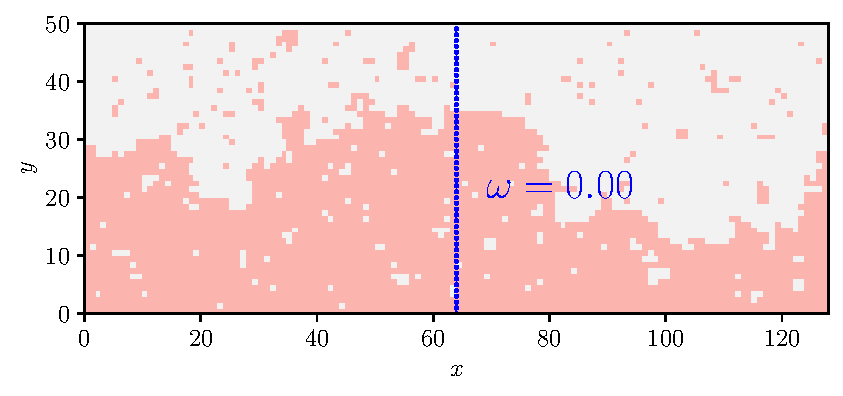
\includegraphics[width=\linewidth]{intro/cis-ising-f-000.pdf}
	\end{minipage}%
	\begin{minipage}[t]{0.5\linewidth}
		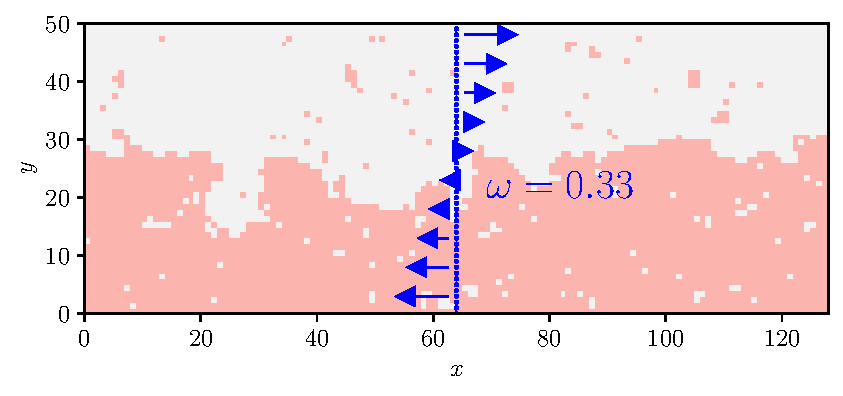
\includegraphics[width=\linewidth]{intro/cis-ising-f-033.pdf}
	\end{minipage}
	\centering
	\begin{minipage}[t]{0.5\linewidth}
		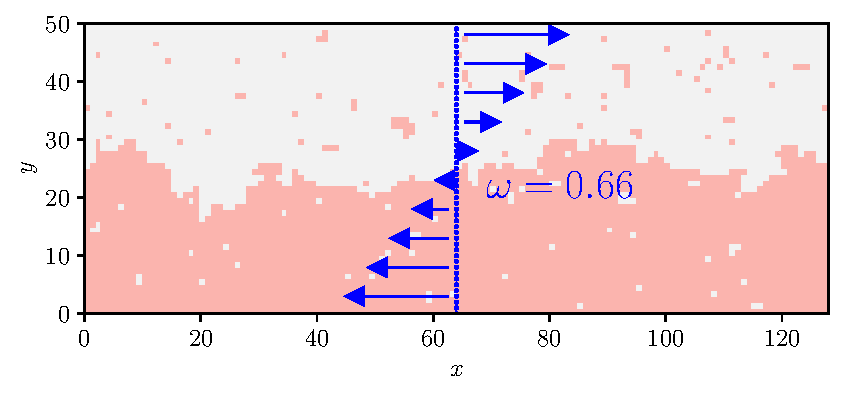
\includegraphics[width=\linewidth]{intro/cis-ising-f-066.pdf}
	\end{minipage}
	\caption{Photos d'un système d'Ising en fonction du cisaillement  \ref{eq-cisaillement} via des simulations de Monte Carlo avec un algorithme de Kawasaki. Ledit algorithme sera expliqué plus en détail au chapitre \ref{chap-sim}.}
    \label{snap-ising-shear}	
\end{figure}  


\section{Conclusion}

Nous avons présenté les modèles standards des transitions de phase et avons étudié l'importance de l'ensemble thermodynamique dans ces systèmes. Dans l'ensemble grand-canonique où le paramètre d'odre n'est pas conservé, les équations dynamiques du modèle A \ref{MA} appliqués au champ $\phi(\mx,t)$ permettent de calculer la fonction de corrélation du système pour le modèle $\phi^4$. Le modèle $\phi^4$ permet de basculer naturellement vers un modèle d'interface $h(\mx,t)$ qui réduit la dimensionalité des équations et permet de n'étudier qu'une partie précise du problème. Nous avons expliqué comment passer d'un modèle de champ à un modèle d'interface, en dérivant des équations très similaires entre les deux modèles.

Lorsques la longueur de corrélation des fluctuations deviennent de l'ordre de grandeur de la taille du système, la contrainte influe sur l'énergie libre totale. On a démontré que l'énergie libre libre se décompose alors en un terme de volume, un terme de surface dépendant des conditions aux bords, et d'un terme d'excès. La dérivée de l'énergie libre en fonction de la taille du système nous donne une pression de confinement, qui dans les systèmes critiques, s'appelle force de Casimir. Nous avons expliqué commennt mesurer cette force par une intégration sur le paramètre d'ordre, dans le cas où il n'est pas possible de calculer analytiquement l'énergie libre du système.

Une attention particulière a été portée aux ensembles thermodynamiques. Bien que l'hypothèse de l'équivalence des ensembles thermodynamiques implique que les systèmes se comportent identiquement à l'équilibre pour des systèmes thermodynamiques, la dynamique des systèmes confinés est particulièrement différente dans les deux cas. De plus, nous avons vu que seul l'ensemble canonique permettait, grâce à une dynamique locale, d'obtenir des systèmes hors-équilibre. Expérimentalement, la manière la plus simple est de cisailler les parois du système afin d'induire un flux stationnaire. 